\documentclass[11pt,a4paper]{article}
\usepackage{alex-report}
\ReportSetup{DSpecM1D scientific validation}{Study 1}{3 November 2026}
\hypersetup{pdftitle={DSpecM1D study 1: source-shell traces and derivative checks}}
\begin{document}
\ReportTitle{Source-shell traces and derivative checks}{Isolated DSpec--YSpec study; no new Sobolev formulation}
\textbf{Finding.} The dominant raw native-array difference occurs at the source radius and compares different trace conventions. YSpec repeats one public source-radius value in both native slots; that value closely tracks the DSpec outer trace, while the DSpec inner trace differs. This is not a matched-trace accuracy error or evidence of a numerical infinity. The supported smooth-perturbation derivative test passes at two step sizes. Continuum singularity and global function-space questions remain unresolved.

\section{Problem and scope}
The fixture is the attenuated anisotropic PREM transverse-velocity traveltime case: source depth 29.5 km, receiver depth 3 km, 60-degree separation, 1000--1200 s window, 40 s taper, and the existing 2/4/8/10 mHz filter. All 35 frequency bins (7--41), full gravity, full radial systems, moment tensor, damping and normalization were retained. The receiver is on the solid side of the solid--fluid boundary at radius 6,368,000 m. The source radius 6,341,500 m is inside a material layer; the source-aligned SEM split is not a material jump.

The L200 comparison uses NQ6 and mesh-step parameter $h=0.02035382429229197$. A shared grid contains 168 fixed physical probes at 14 great-circle locations, with explicit material and radial-trace identifiers. Twenty-eight exact source-shell probe traces are unavailable through YSpec's public sampling interface. The raw native outputs remain unmasked. Neither section sample norms nor finite grid values establish a three-dimensional $L^2$ or $H^1$ limit.\footnote{Point-source sensitivity examples motivate this caution: A. Fichtner, H.-P. Bunge and H. Igel, \emph{The adjoint method in seismology II} (2006), \url{https://www.geophysik.uni-muenchen.de/~igel/EGU2007/Material/Fichtner/adjoint_2_rev.pdf}. Those examples do not prove divergence in this fixture.}

\section{The source-shell comparison}
At along-path angle 0.447761 degrees, the largest raw along-section difference has the following values, in s\,m$^{-3}$:
\begin{center}\begin{tabular}{lr}\toprule
Sample & Value \\\midrule
DSpec inner source-shell trace & $5.26111867\times10^{-15}$ \\
DSpec outer source-shell trace & $1.04578547\times10^{-14}$ \\
YSpec value repeated in both native slots & $1.04579166\times10^{-14}$ \\\bottomrule
\end{tabular}\end{center}
The raw difference is 49.6928\% of the maximum absolute DSpec value over the full along section. It is preserved, but the two sides cannot be treated as interchangeable ordinary point samples. Separate source-contact terms are not included in these regular volume-kernel arrays. A new $H^1$ gradient or regularization has not been implemented.

\begin{figure}[H]\centering
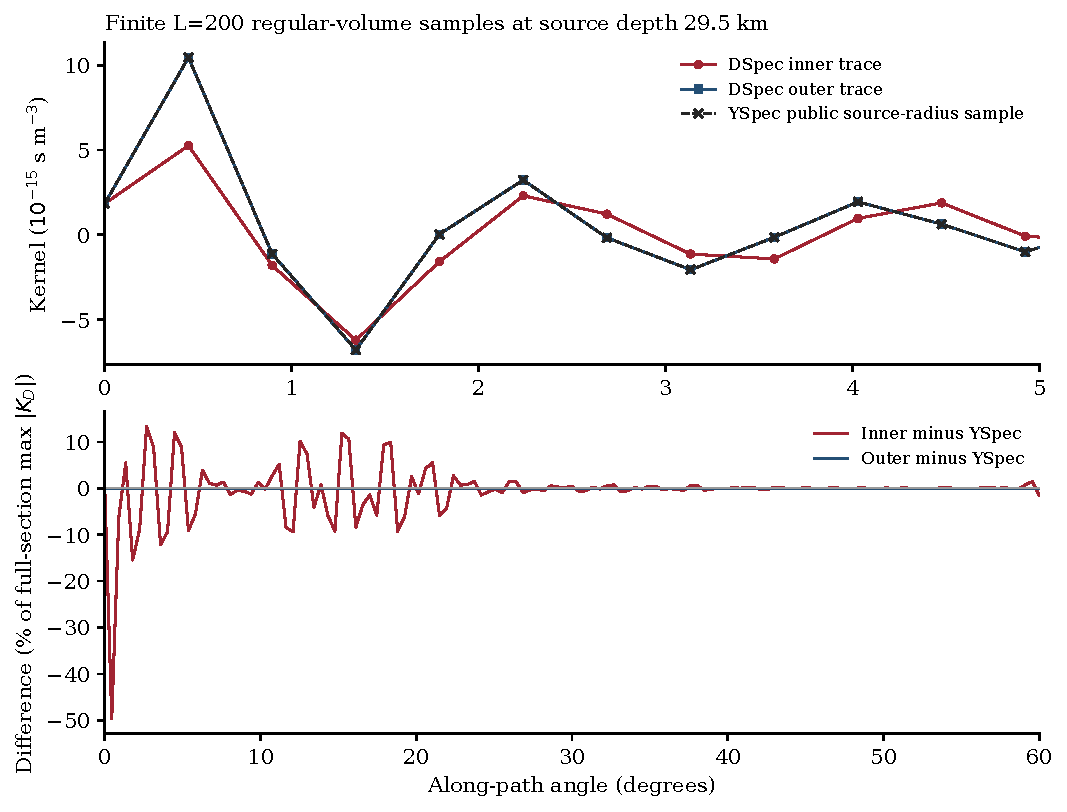
\includegraphics[width=.96\linewidth]{figures/study1-source-traces.pdf}
\caption{Actual finite-L regular-volume source-shell samples. The upper panel shows the source-neighbourhood sample curves; the lower panel retains the full along-path differences, normalized independently by the full along-section DSpec maximum. Lines connect samples for display. Contact terms and undefined continuum point values are not represented by these curves.}
\end{figure}

\section{Section diagnostics and refinement controls}
The table gives discrete sample $\ell^2$ differences in percent, using DSpec's sample norm as the denominator. It is not a volume norm. Removing a cohort for a diagnostic does not turn the remaining statistic into a global error bound.
\begin{center}\begin{tabular}{lrr}\toprule
Sample cohort & Along (\%) & Across (\%) \\\midrule
All native samples & 12.273754 & 3.676496 \\
Source-radius samples (unmatched traces) & 33.013378 & 36.276463 \\
Off-source-radius samples & 0.008913 & 0.003713 \\
\bottomrule\end{tabular}\end{center}
Changing DSpec's mesh scale from 0.9 to 0.8 changes the step parameter from 0.02035382429229197 to 0.018092288259815084 (ratio $8/9$). The fixed-probe kernel change is $3.785\times10^{-9}$ relative sample $\ell^2$, and the saved whole velocity-trace change is $4.543\times10^{-9}$. Tightening YSpec's ODE tolerance from $10^{-5}$ to $10^{-7}$ changes its 140 exposed fixed-probe kernels by $6.766\times10^{-6}$ and its whole velocity trace by $1.796\times10^{-5}$. These are one refinement pair per solver, not asymptotic certificates.

All evaluated samples were finite. The nearest native source and receiver distances are already zero on both radial meshes, so these data do not form a shrinking-distance sequence. A separate DSpec-field/YSpec-weight counterfactual is recorded in the machine-readable evidence; it does not supply unavailable YSpec unit fields or define unique physical attribution.

\section{A genuine three-dimensional derivative action}
The low-degree control uses L3, NQ8 and $h=0.05$. The compact radial profile is $q(r)=\sin^2[\pi(r-5.3\,\mathrm{Mm})/(0.5\,\mathrm{Mm})]$ on 5.3--5.8 Mm and zero elsewhere. This profile is $C^1$ across its support endpoints and is separated from the source and receiver radii by at least 541.5 km. It changes $\ln v_s$ at fixed $v_p$, density and effective Q.

The full angular quadrature has 91 directions and weights summing to $4\pi$; its 157 one-sided radial samples cover the entire perturbation support. The action $\int Kq\,r^2\,dr\,d\Omega$ is therefore a three-dimensional action, not a section integral. The DSpec value is $-106.023590250$ s, and the YSpec value using its own waveform-derived weights is $-106.023536482$ s. Only DSpec was independently tested with perturbed full-forward solves: the concrete YSpec model API does not expose the identical continuous perturbation callback.

For each $\epsilon$, the centred full-forward difference is paired with the \emph{unperturbed baseline} adjoint source. Meshes, parameters, source, receiver side and frequency grids match exactly within the pair; the perturbed runs' own weights are not used for this comparison.
\begin{center}\begin{tabular}{rrr}\toprule
$\epsilon$ & Full-forward derivative (s) & Relative difference \\\midrule
$1\times10^{-4}$ & -106.023587916 & $2.201\times10^{-8}$ \\
$5\times10^{-5}$ & -106.023590011 & $2.247\times10^{-9}$ \\
\bottomrule\end{tabular}\end{center}
Both relative differences and the inter-step change ($1.976\times10^{-8}$) pass the predeclared $2\times10^{-4}$ limit. This tests the selected discrete derivative for a support away from singular locations. An independent matrix/tangent derivative calculation and near-contact perturbation tests were not performed.

\section{Review, provenance and next study}
Ten solver jobs completed with unchanged tracked inputs and verified cleanup. Peak observed numerical use was nine threads and 1.2523 GiB. The separate checker completed with return code zero against an immutable producer-state snapshot; its scientific FD status is PASS. The user-space watchdog is not kernel aggregate enforcement.

Sol independently reviewed the saved numerical evidence after study 1. The review accepts the trace-contract interpretation and derivative evidence; it does not prove global regularity, absence of every implementation defect, or convergence of singular pointwise values. Study 2 will vary spatial resolution and degree separately, retain source-shell traces as a distinct cohort, and include an above-L200 control with bounded diagnostic sampling.

\footnotesize
Machine-readable report SHA-256: \texttt{040252a3415789dec6935a7d3681af3a48ae5c6a34f2348f55d1b1630f945d43}.\\
Raw archive SHA-256: \texttt{f1f60203890f4e63296e1b8dc1b63cf64f6fce6d47d0067c80e39b92533ac1e5}.\\
After-results review SHA-256: \texttt{d73b839a4fad25a66a8a52fcae1eb9507c21437156a80b4a3cfe19a9dfa2ee95}.
\normalsize
\end{document}
